% filepath: c:\Users\kuba-\Desktop\simple_graph_tool_xdf\src\eeg\reportPendulum.tex
\documentclass[12pt]{article}
\usepackage[T1]{fontenc} % Use T1 font encoding
\usepackage[utf8]{inputenc} % Ensure UTF-8 encoding
\usepackage[polish]{babel} % Enable Polish language support
\usepackage{amsmath}
\usepackage{graphicx}
\usepackage{booktabs}
\usepackage{float}
\usepackage[margin=2.5cm]{geometry}
\usepackage{siunitx}
\usepackage{titlesec}
\titlespacing*{\subsection}{0pt}{*0.5}{*0.5} % Adjusts spacing before and after subsections
\usepackage{caption}
\usepackage{lmodern}
\usepackage{placeins} % For FloatBarrier
\usepackage{hyperref} % For hyperlinks in the document

\title{Odległość Ogniskowa cieńkich soczewek}
\date{}

\begin{document}

% --------------------------- STRONA TYTUŁOWA --------------------------
\begin{titlepage}
    \centering
    \Large
    \textbf{DYDAKTYCZNE LABORATORIUM FIZYKI} \\
    \vspace{0.2cm}
    \textbf{UNIWERSYTET RADOMSKI}\\
    im. Kazimierza Pułaskiego w Radomiu \\
    
    \vspace{1.5cm}
    \begin{flushleft}
        \textbf{Wydział:} {WTEiI} \\
        \textbf{Kierunek:} Informatyka \\
        \textbf{Rok Akademicki:} 2024/2025 \\
        \textbf{Semestr:} II \\
        \textbf{Grupa:} 3 \\
        \textbf{Zespół:} 2 \\
        \textbf{Data:} 11.03.2025 \\
        \textbf{Prowadzący ćwiczenie:} dr M. Gzik - Szumiata \\
    \end{flushleft}
    
    \vspace{1cm}
    \begin{flushleft}
        \textbf{Nr ćwiczenia:} 4 \\
        \textbf{Temat ćwiczenia:} \\
        \textbf{Odległość Ogniskowa cieńkich soczewek} \\
    \end{flushleft}
    
    \vspace{1cm}
    \begin{flushleft}
        \textbf{Wykonujący ćwiczenie:}
        \begin{itemize}
            \item Jakub Oleszczuk
            \item Mikołaj Majewski
            \item Mateusz Ofiara
        \end{itemize}
    \end{flushleft}

    \vfill
    \begin{flushleft}
        \textbf{Oceny:} \\
        1.\hspace{2cm}2.\hspace{2cm}3.
    \end{flushleft}
\end{titlepage}

% --------------------------- TREŚĆ SPRAWOZDANIA --------------------------
\section*{Wstęp}
Celem ćwiczenia było wyznaczenie ogniskowej soczewki skupiającej z wykorzystaniem metody Bessela. 
Polegało ono na przygotowaniu lampy oświetlającej blaszkę z wyciętym kształtem za którym dodatkowo 
stała w pewnej odległości soczewka oraz dalej blaszka (tzw. ekran) na którą padało światło.
Wykonane zostały pomiary w wielu punktach pomiarowych gdzie dzięki ławie optycznej zmienialiśmy 
odległości pomiędzy blaszką a ekranem aby wyznaczyć “ogniskowe” naszej soczewki.

\section*{Tabele}
\begin{table}[H]
    \centering
    \caption{Tabela pomiarowa dla obrazu powiększonego}
    \begin{tabular}{|c|c|c|c|c|c|c|c|c|}
        \hline
        \textbf{l} & \textbf{$x_1$} & \textbf{$x_2$} & \textbf{$x_3$} & \textbf{$x_4$} & \textbf{$x_5$} & \textbf{y} & \textbf{$\bar{x}$} & \textbf{f} \\ \hline
        170           & 38       & 39        & 38.5       & 38.5        & 39       & 133        & 38.6       & 29.917        \\ \hline
        159           & 40       & 40        & 40       & 40        & 40       & 119        & 40       & 29.937        \\ \hline
        148           & 40.5     & 41        & 41       & 41.5        & 41       & 107        & 41       & 29.641        \\ \hline
        137           & 43       & 43.5        & 43.5       & 43.5        & 43.5       & 94        & 43.3       & 29.691        \\ \hline
        126           & 46       & 46.5        & 47.5       & 47        & 47       & 79        & 46.8       & 29.389        \\ \hline
    \end{tabular}
    \captionsetup{font=small, justification=centering}
    \caption*{\textit{Legenda: $l$ - odległość w cm, $x_1, x_2, \dots$ - pomiary w cm, $y$ - odległość obrazu w cm, $\bar{x}$ - średnia wartość pomiarów, $f$ - ogniskowa w cm.}}
\end{table}
\begin{table}[H]
    \centering
    \caption{Tabela pomiarowa dla obrazu pomniejszonego}
    \begin{tabular}{|c|c|c|c|c|c|c|c|c|}
        \hline
        \textbf{l} & \textbf{$x_1$} & \textbf{$x_2$} & \textbf{$x_3$} & \textbf{$x_4$} & \textbf{$x_5$} & \textbf{y} & \textbf{$\bar{x}$} & \textbf{f} \\ \hline
        170           & 132       & 133        & 132.5       & 132.5        & 132.5       & 39        & 132.5       & 30.131        \\ \hline
        159           & 119       & 119        & 119.5       & 119        & 119.5       & 40        & 119.2       & 29.949        \\ \hline
        148           & 108.6     & 108        & 108.5       & 108.5        & 107.5       & 41.5        & 108.22       & 29.996        \\ \hline
        137           & 94       & 93        & 93       & 94        & 94       & 44        & 93.6       & 29.930        \\ \hline
        126           & 79       & 79        & 79       & 79        & 78       & 48        & 78.8       & 29.829        \\ \hline
    \end{tabular}
    \captionsetup{font=small, justification=centering}
    \caption*{\textit{Legenda: $l$ - odległość w cm, $x_1, x_2, \dots$ - pomiary w cm, $y$ - odległość obrazu w cm, $\bar{x}$ - średnia wartość pomiarów, $f$ - ogniskowa w cm.}}
\end{table}

\bfseries{Średnia wartość ogniskowej soczewek wynosi:}
\begin{equation}
    \bar{f} = \frac{\sum f}{n} = 29.841\,cm \pm 0,031 \, \mathrm{cm}
\end{equation}
\textit{gdzie:}
\begin{itemize}
    \item $\sum f$ - suma ogniskowych,
    \item $n$ - liczba pomiarów.
\end{itemize}
\textit{Błąd pomiarowy wynosi: 1cm.}

\section*{Wykres}
\begin{figure}[H]
    \centering
    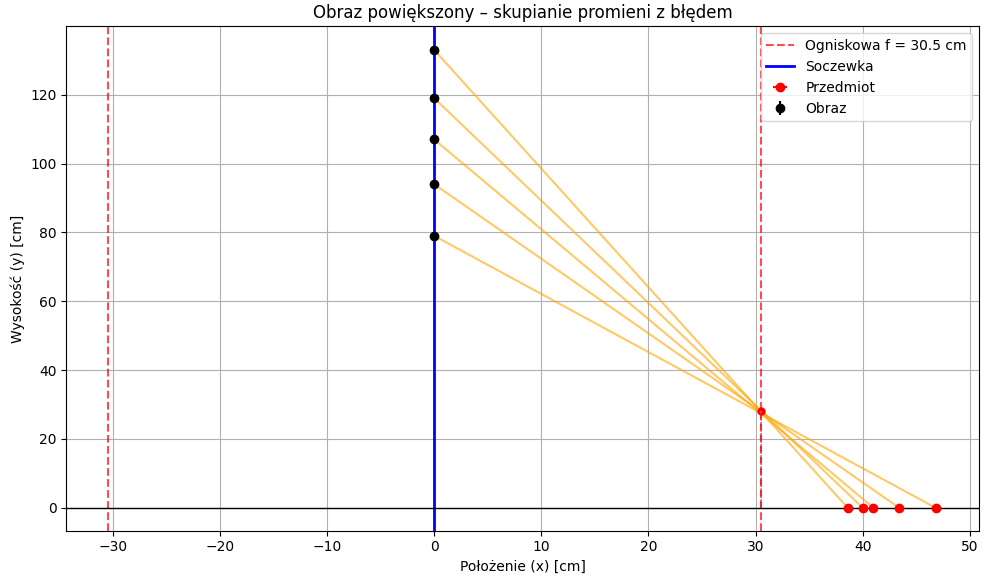
\includegraphics[width=0.8\textwidth]{obraz_pow.png}
    \caption{Graficznie wyznaczenie ogniskowej soczewki dla obrazu powiększonego}
    \label{fig:wykres1}
\end{figure}
\begin{figure}[H]
    \centering
    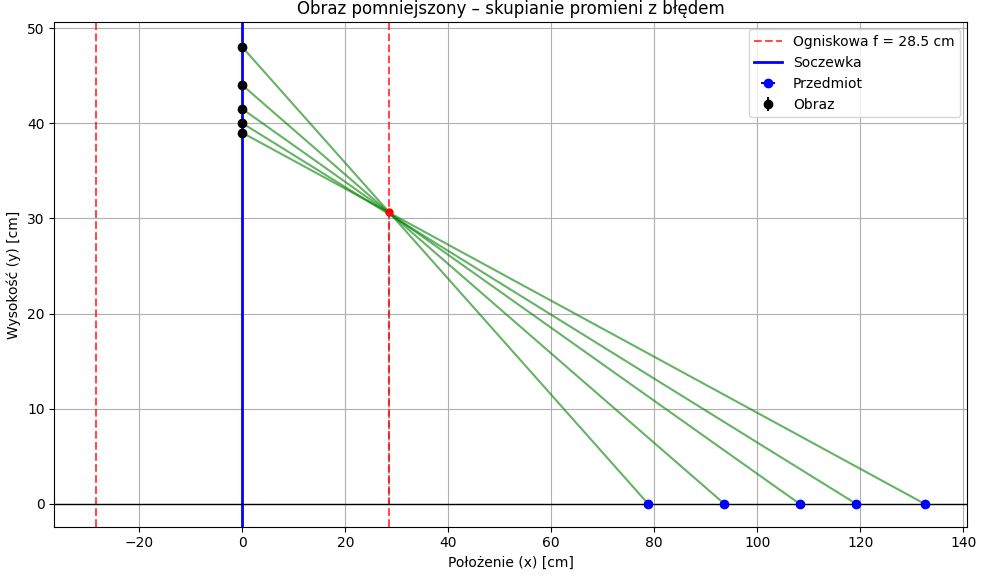
\includegraphics[width=0.8\textwidth]{obraz_pom.png}
    \caption{Graficznie wyznaczenie ogniskowej soczewki dla obrazu pomniejszonego}
    \label{fig:wykres2}
\end{figure}

\clearpage

\section*{Obliczenia}
\begin{equation}
    \frac{1}{f} = \frac{1}{l} + \frac{1}{y}
\end{equation}

\begin{itemize}
    \item $f$ - ogniskowa,
    \item $l$ - odległość soczewki od przedmiotu,
    \item $y$ - odległość soczewki od obrazu.
\end{itemize}

\section*{Wnioski}
Dla ustalonej odległości między przedmiotem (blaszką) a ekranem, możliwe było znalezienie dwóch położeń 
soczewki, w których otrzymujemy ostry obraz na ekranie. Jest to kluczowa cecha metody Bessela, gdzie 
dla jednej ustalonej odległości między przedmiotem a ekranem (L, gdzie L > 4f) pojawiają się dwa różne 
położenia soczewki dające ostry obraz na ekranie.

W pierwszej pozycji soczewka znajduje się bliżej przedmiotu -- wtedy obraz powstaje dalej (za soczewką). 
W drugiej pozycji soczewka znajduje się bliżej ekranu -- wtedy przedmiot znajduje się dalej od soczewki. 
W obu przypadkach spełnione jest równanie soczewki cienkiej:
\[
    \frac{1}{f} = \frac{1}{x} + \frac{1}{y} \quad \text{(gdzie } x + y = L\text{)}
\]

Dla danej wartości L, równanie to może mieć dwa rozwiązania: jedno z większym x i mniejszym y, 
oraz drugie odwrotnie. Oba przypadki dają tak samo ostre obrazy, lecz przy innych pozycjach soczewki. 
Pokazuje to symetryczność działania soczewki skupiającej -- może ona tworzyć obraz zarówno z małego 
przedmiotu znajdującego się blisko niej, jak i z większego, dalszego przedmiotu. W obu przypadkach 
otrzymuje się obraz tej samej wielkości, różniący się jedynie położeniem i odwrotną rolą przedmiotu/obrazu.

Powtarzanie pomiarów dla różnych wartości odległości L (przedmiot--ekran) umożliwiło uśrednienie wyników 
i uzyskanie dokładniejszego, bardziej wiarygodnego wyniku ogniskowej soczewki.

Przeprowadzone ćwiczenie pozwoliło na lepsze zrozumienie zasad rządzących tworzeniem obrazów przez 
soczewki skupiające oraz praktyczne wykorzystanie tych zasad do pomiarów optycznych.

Ćwiczenie pokazało też jak ważne jest precyzyjne ustawienie soczewki i ekranu, aby uzyskać ostry obraz,
co może być to trudne w praktyce, bo wymaga to dużej dokładności i cierpliwości, przy pomiarze odległości
miarą zwijaną dochodzą błędy pomiarowe przy każdym pomiarze, co może prowadzić do niedokładnych wyników.

\end{document}
